\clearpage
\setcounter{page}{1}
\maketitlesupplementary
% The supplement is one appendix: its sections are numbered A.1, A.2, ... and its tables, figures and
% equations A1, A2, ..., so that no number of the supplement can be confused with one of the paper.
\setcounter{section}{0}\renewcommand{\thesection}{A.\arabic{section}}
\setcounter{table}{0}\renewcommand{\thetable}{A\arabic{table}}
\setcounter{figure}{0}\renewcommand{\thefigure}{A\arabic{figure}}
\setcounter{equation}{0}\renewcommand{\theequation}{A\arabic{equation}}
% hyperref anchors: without these, the restarted counters reuse the anchors of the paper (section.1, table.1, ...)
% and a link to Sec. A.1 jumps to Sec. 1.
\renewcommand{\theHsection}{A.\arabic{section}}\renewcommand{\theHtable}{A\arabic{table}}%
\renewcommand{\theHfigure}{A\arabic{figure}}\renewcommand{\theHequation}{A\arabic{equation}}%


\section{Spectral Formulation of the Image Formation}
\label{sec:supp-image-formation}
The camera sensor has a certain spectral sensitivity $S(\lambda)$~\cite{akkaynak2017space,
akkaynak2018revised, Darrodi:15, pharr2023physically,
toivonen2020practical} and measures the spectral radiant flux as \cite{space-of-spectral-sensitivity-2013}
\begin{align*}
    S(\lambda)\Phi(\vbu,\lambda) = \int_{\mathcal{I}_{\vbu}}S(\lambda)E(\vbp,\lambda)\odif{\vbp}.
\end{align*}
This spectral formulation requires knowledge of the camera's spectral sensitivity
$S(\lambda)$ which is difficult to recover in practice because it
requires specialized equipment \cite{akkaynak2017space, Darrodi:15, toivonen2020practical}. Tri-color (RGB) renderers avoid this by working directly with per-channel quantities~\cite{Finlayson-PAMI-2017, rgb}.
Let $\Lambda_c$ be the set of wavelengths associated with the channel $c\in\{r,g,b\}$.
The per-channel radiant flux measured by the sensor in pixel $\vbu$ becomes
\begin{align*}
    &\Phi_c(\vbu) \coloneqq \int_{\mathcal{I}_{\vbu}}\underbrace{\int_{\Lambda_c}S_c(\lambda)E(\vbp,\lambda)\odif{\lambda}}_{\eqqcolon E_c(\vbp)}\odif{\vbp}\nonumber\\
    &=\int_{\mathcal{I}_{\vbu}}\int_{\calOmega(\vbp)}\underbrace{\int_{\Lambda_c}S_c(\lambda)L(\vbx(\vbp,\vbomega),\vbomega_o(\vbp,\vbomega),\lambda)\odif{\lambda}}_{\eqqcolon L_c(\vbx(\vbp,\vbomega),\vbomega_o(\vbp,\vbomega))}\nonumber\\
    &\qquad\qquad\qquad\qquad\qquad\qquad\qquad\cdot\cos\theta(\vbomega)\odif{\vbomega}\odif{\vbp}\nonumber,
\end{align*}
where Fubini's theorem~\cite{heuser2004} is used to swap the order of the integrals.
In the main text and in the following, all quantities are per color channel and the channel index $c$ is omitted.


\section{Geometric Camera Models and the Pinhole Aperture}
\label{sec:supp-pinhole-radiometry}
\label{sec:supp-camera-models}
The pinhole model can be constructed from the thin lens model by making the aperture radius infinitesimal so that for each sensor position only a single ray passes through the pinhole $\vbo\in\mathcal{A}$~\cite{pharr2023physically}.
Using the Dirac delta distribution $\delta$, which satisfies the sifting property \cite{Bracewell1966TheFT, pinholedelta}
\begin{align}
\label{eq:sifting}
    \int_{\calOmega(\vbp)} g(\vbomega)\delta(\vbomega-\vbomega_0)\odif{\vbomega} = g(\vbomega_0)
\end{align}
to select the radiance along the single ray direction $\vbomega_0 \coloneqq \vbo - \vbp$ through the pinhole \cite{pinholedelta}, the radiant flux \cref{eq:per-channel-rad-flux} simplifies to
\begin{align}
    &\int_{\mathcal{I}_{\vbu}} \int_{\calOmega(\vbp)} \hspace{-0.3cm}L(\vbx(\vbp,\vbomega),\vbomega_o(\vbp,\vbomega))\cos\theta(\vbomega)\delta(\vbomega-\vbomega_0) \odif{\vbomega}\odif{\vbp}\nonumber\\
    \overset{(\ref{eq:sifting})}&{=} \int_{\mathcal{I}_{\vbu}}L(\vbx(\vbp,\vbomega_0),\vbomega_o(\vbp,\vbomega_0))\cos\theta(\vbomega_0)\odif{\vbp}\label{eq:pinhole-rad-flux} = \Phi(\vbu).
\end{align}
\cref{eq:pinhole-rad-flux} shows that the pinhole model is a pure geometric model and physically incorrect:
a vignetting falloff is missing and every scene point is in perfect focus.

% The camera models are subsections of this section, and their overview is not a numbered table, so that the section
% and table numbers that the submitted paper refers to (Secs. A.1 to A.13, Tabs. A1 to A5) do not change.
The geometric camera models that the radiometric camera lifts are all
models of a pinhole aperture. The radiometric camera uses them through
their back-projection $\vbpi^{-1}$ alone
(\cref{eq:lifted-back-projection}), so it places no condition on how a
model is parameterized. The remainder of this section defines the five
models of \cref{sec:geometric-accuracy}, derives their
back-projections, gives the geometric meaning of their parameters
$\vbTheta_d$, and separates them into \emph{global} and \emph{local}
models. The distinction decides how a model is regularized and how the
vignetting, which is radially symmetric about the principal point
(\cref{sec:vignetting}), is attached to it.
\begin{center}
  \footnotesize\setlength{\tabcolsep}{3pt}
  \begin{tabular*}{\linewidth}{@{\extracolsep{\fill}}llll@{}}
    \toprule
    \textbf{Model} & \textbf{Parameters} $\vbTheta_d$ & \textbf{Scope} & \textbf{Principal point} \\
    \midrule
    Brown--Conrady & $f_x,f_y,\vbc$, 5 coeff. & global & parameter $\vbc$ \\
    OpenCV-14 & $f_x,f_y,\vbc$, 14 coeff. & global & parameter $\vbc$ \\
    Kannala--Brandt & $f_x,f_y,\vbc$, 4 coeff. & global & parameter $\vbc$ \\
    Double Sphere & $f_x,f_y,\vbc$, $\xi,\alpha$ & global & parameter $\vbc$ \\
    Central spline & $\vbd_{ij}$ per node & local & estimated, \cref{eq:supp-axis-fit} \\
    \bottomrule
  \end{tabular*}
\end{center}

\subsection{Global Models}
\label{sec:supp-global-models}
Let the $z$-axis of the camera frame be the optical axis. A
parametric model maps a direction $\vbd=(X,Y,Z)^\top$ of this frame
to a point $(x_d,y_d)$ of the normalized image plane and from there
to the sensor point
\begin{equation}
\label{eq:supp-intrinsics}
    \vbp = \bigl(f_x x_d + c_x,\; f_y y_d + c_y\bigr)^\top,
\end{equation}
with the focal lengths $f_x,f_y$ in pixels and the principal point
$\vbc=(c_x,c_y)^\top$. The models differ in the map
$\vbd\mapsto(x_d,y_d)$, which we write with the angle $\theta$
between $\vbd$ and the optical axis and the azimuth $\varphi$ about
it,
\begin{equation}
\label{eq:supp-angles}
    \theta=\operatorname{atan2}\bigl(\sqrt{X^2+Y^2},Z\bigr),
    \qquad \varphi=\operatorname{atan2}(Y,X).
\end{equation}
All four models are defined by this forward projection. The
back-projection $\vbpi^{-1}$ inverts it: \cref{eq:supp-intrinsics}
gives $(x_d,y_d)$ from $\vbp$, and the inverse of the map
$\vbd\mapsto(x_d,y_d)$, derived below for each model, gives the
direction. We call these models \emph{global}: each of their few
parameters changes the back-projection of every sensor point.

\paragraph{Brown--Conrady.} The model starts from the perspective
projection $(x,y)=(X/Z,\,Y/Z)$, whose radius is
$\rho=\sqrt{x^2+y^2}=\tan\theta$. A lens that is rotationally
symmetric about its optical axis displaces an image point along its
radius, and by symmetry the displaced radius is an odd function of
$\rho$, so that $\rho_d=\rho\,R(\rho)$ with a factor $R$ that is even
in $\rho$. Brown \cite{Brown1966DecenteringDO} truncates its series
after three terms and adds the displacement that Conrady
\cite{Conrady1919DecentredL} derived for lens elements whose centers
are not on a common axis, which is not radial:
\begin{align}
\label{eq:supp-brown-conrady}
    x_d &= x\,R(\rho) + 2p_1xy + p_2(\rho^2+2x^2),\nonumber\\
    y_d &= y\,R(\rho) + p_1(\rho^2+2y^2) + 2p_2xy,\\
    R(\rho) &= 1+k_1\rho^2+k_2\rho^4+k_3\rho^6.\nonumber
\end{align}
The radial coefficients $k_1,k_2,k_3$ describe barrel distortion
where $R<1$ and pincushion distortion where $R>1$. The tangential
coefficients $p_1,p_2$ are the components of the decentering along
the two image axes. \Cref{eq:supp-brown-conrady} has no closed-form
inverse. We solve it for $(x,y)$ iteratively from
$(x,y)=(x_d,y_d)$, which has a unique solution where the distortion is
monotonic, \ie where $\rho\,R(\rho)$ increases with $\rho$, and the
back-projection is
$\vbpi^{-1}(\vbp)=(x,y,1)^\top/\lVert(x,y,1)\rVert$. Since
$\rho=\tan\theta$ diverges for $\theta\to90^\circ$, the model cannot
represent a field of view of $180^\circ$.

\paragraph{OpenCV-14.} The 14-parameter model of OpenCV
\cite{opencv_library} extends \cref{eq:supp-brown-conrady} by three
effects. First, the radial factor becomes a rational function,
\begin{equation}
\label{eq:supp-rational}
    R(\rho) = \frac{1+k_1\rho^2+k_2\rho^4+k_3\rho^6}{1+k_4\rho^2+k_5\rho^4+k_6\rho^6},
\end{equation}
which tends to a constant for large $\rho$, where a polynomial
diverges, and therefore follows a wide-angle lens further toward the
image border. Second, thin-prism terms describe lens elements that
are tilted against the optical axis, which displace the image by even
powers of the radius along a fixed direction:
\begin{align}
\label{eq:supp-thin-prism}
    x' &= x\,R(\rho) + 2p_1xy + p_2(\rho^2+2x^2) + s_1\rho^2+s_2\rho^4,\nonumber\\
    y' &= y\,R(\rho) + p_1(\rho^2+2y^2) + 2p_2xy + s_3\rho^2+s_4\rho^4.
\end{align}
Third, the sensor may be tilted against the plane perpendicular to
the optical axis. With the rotation
$\mathrm{T}=\mathrm{R}_y(\tau_y)\,\mathrm{R}_x(\tau_x)$ of the sensor
by the angles $\tau_x,\tau_y$ about the image axes, with the entries
$T_{ij}$, the point is mapped by the homography
\begin{equation}
\label{eq:supp-tilt}
    \lambda\begin{pmatrix}x_d\\y_d\\1\end{pmatrix}
    = \begin{pmatrix} T_{33} & 0 & -T_{13}\\ 0 & T_{33} & -T_{23}\\ 0 & 0 & 1\end{pmatrix}
    \mathrm{T}\begin{pmatrix}x'\\y'\\1\end{pmatrix},
\end{equation}
which rotates the image plane into the plane of the tilted sensor
and projects it back along the optical axis, so that the principal
point stays where the optical axis meets the sensor. The 14
parameters are $k_1,\dots,k_6$, $p_1,p_2$, $s_1,\dots,s_4$ and
$\tau_x,\tau_y$, and $k_4=\dots=\tau_y=0$ is the Brown--Conrady
model. For the back-projection, \cref{eq:supp-tilt} is inverted in
closed form, as a homography, and \cref{eq:supp-thin-prism} is then
solved for $(x,y)$ iteratively as above. The model distorts
the perspective projection as well and shares its limit of
$180^\circ$.

\paragraph{Kannala--Brandt.} A fisheye lens is not designed to image
a direction at the radius $\tan\theta$ of the perspective projection,
but at a radius that stays finite at $\theta=90^\circ$, \eg $\theta$
(equidistant), $2\tan\frac{\theta}{2}$ (stereographic) or
$2\sin\frac{\theta}{2}$ (equisolid angle). All of these, and the
perspective projection itself, are odd functions of $\theta$.
Kannala and Brandt \cite{kannala-brandt} therefore model a
rotationally symmetric lens by an odd polynomial in $\theta$, whose
linear coefficient is absorbed by the focal length:
\begin{align}
\label{eq:supp-kannala-brandt}
    (x_d,y_d) &= r(\theta)\,(\cos\varphi,\sin\varphi),\nonumber\\
    r(\theta) &= \theta+k_1\theta^3+k_2\theta^5+k_3\theta^7+k_4\theta^9,
\end{align}
with $\theta$ and $\varphi$ of \cref{eq:supp-angles}. The first term
is the equidistant projection, and $k_1,\dots,k_4$ describe the
deviation of the lens from it. The model has no decentering terms.
For the back-projection, the azimuth is that of the image point,
$\varphi=\operatorname{atan2}(y_d,x_d)$, and the angle is the root of
$r(\theta)=\sqrt{x_d^2+y_d^2}$, which we find iteratively
from $\theta=\sqrt{x_d^2+y_d^2}$ and which is unique where $r$ is
monotonic. Then
\begin{equation}
    \vbpi^{-1}(\vbp)=(\sin\theta\cos\varphi,\;\sin\theta\sin\varphi,\;\cos\theta)^\top .
\end{equation}
Since $\theta$ is not restricted to less than $90^\circ$, the model
represents fields of view of $180^\circ$ and more.

\paragraph{Double Sphere.} The model of Usenko \etal
\cite{double-sphere} is constructed geometrically. The direction is
projected onto a unit sphere about the center of projection, which
gives $\vbd/d_1$ with $d_1=\lVert\vbd\rVert$. This point is expressed
in the frame of a second unit sphere whose center is displaced by
$\xi$ along the optical axis, where it is
$(X,Y,Z+\xi d_1)^\top/d_1$, and is projected onto the second sphere
by dividing by its norm $d_2/d_1$,
\begin{equation}
    d_2=\sqrt{X^2+Y^2+(\xi d_1+Z)^2}.
\end{equation}
Finally, the point $(X,Y,Z+\xi d_1)^\top/d_2$ on the second sphere is
projected perspectively from a center that is displaced by
$\frac{\alpha}{1-\alpha}$ behind the center of this sphere, which
gives
\begin{equation}
\label{eq:supp-double-sphere}
    (x_d,y_d) = \frac{(X,Y)}{\alpha d_2+(1-\alpha)(\xi d_1+Z)}.
\end{equation}
The parameter $\xi$ is thus the distance between the two spheres and
$\alpha\in[0,1]$ the position of the final center of projection, and
$\xi=0$, $\alpha=0$ is the perspective projection. Both describe a
rotationally symmetric lens, and the model has no decentering terms.
Unlike the three models above, it has a closed-form inverse. With
$\rho^2=x_d^2+y_d^2$,
\begin{align}
\label{eq:supp-double-sphere-inverse}
    m_z &= \frac{1-\alpha^2\rho^2}{\alpha\sqrt{1-(2\alpha-1)\rho^2}+1-\alpha},\nonumber\\
    \vbpi^{-1}(\vbp) &= \frac{m_z\xi+\sqrt{m_z^2+(1-\xi^2)\rho^2}}{m_z^2+\rho^2}
    \begin{pmatrix}x_d\\y_d\\m_z\end{pmatrix}
    -\begin{pmatrix}0\\0\\\xi\end{pmatrix},
\end{align}
which follows from inverting the three steps in reverse order: the
first line intersects the ray of the shifted perspective projection
with the second sphere, and the second line intersects the ray from
the center of the second sphere through this point with the first
sphere. The inverse is a unit vector, and it is defined where
$(2\alpha-1)\rho^2\le1$, which bounds the image radius for
$\alpha>\frac{1}{2}$. The model represents fields of view beyond
$180^\circ$.

\subsection{The Local Model}
\label{sec:supp-local-model}
The central generic model of Schöps \etal \cite{10000params} has no
projection function with physical parameters. It stores the
back-projection itself: directions at the nodes of a regular lattice
over the sensor, interpolated by a bicubic B-spline
\cite{piegl1997nurbs} and normalized. With the control directions
$\vbd_{ij}\in\mathbb{R}^3$ at the nodes $(i,j)$ and the cubic
B-spline basis functions $N_{i,3}$, $N_{j,3}$ over the lattice,
\begin{equation}
\label{eq:supp-spline-lens}
    \hat{\vbd}(\vbp) = \frac{\tilde{\vbd}(\vbp)}{\lVert\tilde{\vbd}(\vbp)\rVert},
    \quad
    \tilde{\vbd}(\vbp) = \sum_{i,j}N_{i,3}(p_x)\,N_{j,3}(p_y)\,\vbd_{ij},
\end{equation}
and $\vbTheta_d=\{\vbd_{ij}\}$. On the Sigma 14\,mm, for example, the
lattice has $35\times25$ nodes at a spacing of about 160 pixels. We
call this model \emph{local}: a cubic basis function is nonzero over
four cells of the lattice, so $\hat{\vbd}(\vbp)$ depends only on the
$4\times4$ control directions around $\vbp$, and a control direction
changes the back-projection only in the $4\times4$ cells around its
node. The model is given by its back-projection and not, as the
global models are, by its forward projection, which has no closed
form. Where a projection is needed, as for the reprojection errors of
\cref{sec:geometric-accuracy}, we invert
\cref{eq:supp-spline-lens} numerically by Levenberg--Marquardt
iterations; a second spline regressed to the inverse is an
alternative, and it is local as well.

The locality has three consequences for the calibration.
\emph{First}, the model can follow a distortion that no global model
describes, but a node is determined only by the photosites in its
own support. Nodes at the border of the lens coverage, which few
photosites see, are therefore not determined by the data, whereas
the parameters of a global model are determined by the whole image.
This is why the central spline, and no other model, is regularized
(\cref{sec:optimization}). \emph{Second}, the model has no
distinguished camera frame: rotating every control direction by a
rotation $\mathrm{R}$ and every pose by its inverse changes no ray
in the scene. A global model does not have this gauge freedom, since
its frame is fixed by its optical axis
(\cref{sec:supp-gauge-freedoms}). \emph{Third}, and for the same
reason, the model has no principal point. The intrinsics of
\cref{eq:supp-intrinsics} do not enter \cref{eq:supp-spline-lens},
which is defined over the sensor directly, so the point about which
the vignetting is symmetric has to be estimated
(\cref{sec:supp-vignetting-center}).

\subsection{The Center of the Vignetting}
\label{sec:supp-vignetting-center}
The vignetting $V$ of \cref{sec:vignetting} is radially symmetric
about a point $\vbc$ of the sensor. The vignetting of a lens is
symmetric about its optical axis, so $\vbc$ has to be the sensor
point that images the axis, which in general is not the center of
the sensor.

\paragraph{Global models.} The principal point of
\cref{eq:supp-intrinsics} is this point by definition: each of the
four models projects the direction of the optical axis,
$\vbd=(0,0,1)^\top$, to $(x_d,y_d)=(0,0)$ and thus to $\vbp=\vbc$.
We center the vignetting at the principal point of the geometric
start.

\paragraph{The local model.} For the central spline, we estimate the
optical axis as the axis about which the camera is closest to
radially symmetric. Let
\begin{equation}
\label{eq:supp-symmetric-camera}
    \vbpi_{\text{sym}}(\vbd)
    \coloneqq \vbc' + r(\theta)\begin{pmatrix} f_x\cos\varphi\\ f_y\sin\varphi\end{pmatrix},
    \quad
    r(\theta)=\theta+\sum_{k=1}^{4}\kappa_k\theta^{2k+1},
\end{equation}
be the projection of a radially symmetric camera, with $\theta$ and
$\varphi$ of \cref{eq:supp-angles}: the model of
\cref{eq:supp-kannala-brandt} with its own focal lengths $f_x,f_y$,
principal point $\vbc'$ and coefficients $\vbkappa$. We regress this
camera and a rotation $\mathrm{R}\in SO(3)$ to the rays of the
spline,
\begin{equation}
\label{eq:supp-axis-fit}
    \min_{\mathrm{R},\,\vbc',\,f_x,\,f_y,\,\vbkappa}\;
    \sum_{\vbp\in\mathcal{R}}
    \bigl\lVert \vbp-\vbpi_{\text{sym}}\bigl(\mathrm{R}\,\hat{\vbd}(\vbp)\bigr)\bigr\rVert^{2},
\end{equation}
where $\mathcal{R}$ are the pixels in which the geometric start is
defined. We minimize it by Levenberg--Marquardt iterations, first
with the coefficient $\kappa_1$ alone and then with one more
coefficient at a time, each from the previous minimum, which keeps
the higher orders from folding the profile at the image border. The
symmetric camera is not used as a camera model. Its role is to
locate the axis: at the minimum, $\mathrm{R}^\top(0,0,1)^\top$ is the
axis about which the rays of the spline are closest to symmetric,
the optical axis of the lens, and $\vbc'$ is the sensor point that
images it. A lens that is not symmetric about any axis leaves a
residual in \cref{eq:supp-axis-fit}, but the axis remains defined as
its minimizer.

We then turn the camera frame onto this axis. Every control
direction is rotated, $\vbd_{ij}\leftarrow\mathrm{R}\,\vbd_{ij}$,
which rotates every ray of \cref{eq:supp-spline-lens} by
$\mathrm{R}$, since the normalization commutes with a rotation, and
every pose $(\mathrm{R}_k,\vbt_k)$ from the world to the camera
becomes $(\mathrm{R}\mathrm{R}_k,\mathrm{R}\vbt_k)$. This uses the
gauge freedom of the local model and changes no ray in the scene.
Afterwards the $z$-axis of the camera frame is the optical axis, and
$\vbc\coloneqq\vbc'$ is the principal point of the spline camera,
with the same meaning as that of a global model. The regression is
done once, on the geometric start. In our experiments it turns the
frame of the spline starts by $0.2^\circ$ to $1.6^\circ$, and the
principal point lies 8 to 25 pixels from the center of the sensor.

\paragraph{During the refinement.} For every model, $\vbc$ is held
at this start value and is not a parameter of the refinement, and
the gauge $V(\vbc)=1$ between the vignetting and the lighting is
fixed there (\cref{sec:supp-gauge-freedoms}). The rotation gauge of
the spline camera is fixed with respect to the same axis: the held
tangent coordinates of \cref{sec:supp-gauge-freedoms} are those of
the node whose direction is closest to it.


\section{Thin Lens Equivalence}
\label{sec:supp-thin-lens-equiv}
Let $\vbpi^{-1}$ be the perspective back-projection,
$\hat{\vbd}(\vbp)=\frac{\vbo-\vbp}{\lVert\vbo-\vbp\rVert}$, and let the
focus surface be the plane at the object distance $s$ from $\vbo$,
perpendicular to the optical axis. The ray of $\vbp$ meets this plane
at the distance $t(\vbp)=\frac{s}{\cos\theta(\vbp)}$ from $\vbo$, where
$\theta(\vbp)$ is the angle between $\hat{\vbd}(\vbp)$ and the optical
axis, so $\tau(\vbp)=\frac{\cos\theta(\vbp)}{s}$ and
$\vbx_f(\vbp)=\vbo+\frac{s}{\cos\theta(\vbp)}\hat{\vbd}(\vbp)$. In the
thin lens model, all rays from $\vbp$ through the aperture meet in the
point in which the ray through the center $\vbo$ of the lens, which is
not refracted, meets the plane of focus \cite{pharr2023physically}.
This point is $\vbx_f(\vbp)$, so that the ray through an aperture point
$\vba$ has the direction
$\frac{\vbx_f(\vbp)-\vba}{\lVert\vbx_f(\vbp)-\vba\rVert}=\vbpi^{-1}(\vbp,\vba)$
of \cref{eq:lifted-back-projection}: without distortion and with a
plane of focus, the radiometric camera is the thin lens.


\section{Inverse Focus Distance}
\label{sec:supp-inverse-depth}
The lifted back-projection \cref{eq:lifted-back-projection} depends
on the focus surface through the distance $t(\vbp)=1/\tau(\vbp)$
from $\vbo$ to the point of focus. We show that its derivative \wrt
the distance $t$ vanishes for a far focus, whereas its derivative
\wrt the inverse distance $\tau$ does not, which is why we
parameterize the focus surface by $\tau$
\cite{unified-inverse-depth,direct-sparse-odometry}. Let
$\vbo = \mathbf{0}$ without loss of generality. With the distance,
\begin{align*}
    &\frac{\partial}{\partial t} \frac{t(\vbp)\hat{\vbd}(\vbp)-\vba}{\lVert t(\vbp)\hat{\vbd}(\vbp)-\vba\rVert}\\
    = &\frac{\hat{\vbd}(\vbp)\lVert t(\vbp)\hat{\vbd}(\vbp)-\vba\rVert - (t(\vbp)\hat{\vbd}(\vbp)-\vba)\frac{t(\vbp)\lVert \hat{\vbd}(\vbp) \rVert^2 - \hat{\vbd}(\vbp)\cdot\vba}{\lVert t(\vbp)\hat{\vbd}(\vbp)-\vba\rVert}}{\lVert t(\vbp)\hat{\vbd}(\vbp)-\vba\rVert^2}
\end{align*}
\begin{align*}
    &\lim_{t\to \infty}\frac{\partial}{\partial t} \frac{t(\vbp)\hat{\vbd}(\vbp)-\vba}{\lVert t(\vbp)\hat{\vbd}(\vbp)-\vba\rVert}\\
    &= \lim_{t\to \infty}\frac{\hat{\vbd}(\vbp)\lVert \hat{\vbd}(\vbp)-\frac{\vba}{t(\vbp)}\rVert - (\hat{\vbd}(\vbp)-\frac{\vba}{t(\vbp)})\frac{\lVert \hat{\vbd}(\vbp) \rVert^2 - \frac{\hat{\vbd}(\vbp)\cdot\vba}{t(\vbp)}}{\lVert \hat{\vbd}(\vbp)-\frac{\vba}{t(\vbp)}\rVert}}{\lVert \hat{\vbd}(\vbp)-\frac{\vba}{t(\vbp)}\rVert^2}\\
    &= 0.
\end{align*}
A focus surface that is far away thus receives no gradient. With the
inverse distance $\tau=\frac{1}{t}$,
\begin{align*}
    &\frac{\partial}{\partial \tau}\frac{-\tau(\vbp)\vba + \hat{\vbd}(\vbp)}{\lVert-\tau(\vbp)\vba + \hat{\vbd}(\vbp)\rVert}\\
    = &\frac{-\vba\lVert \hat{\vbd}(\vbp)-\tau(\vbp)\vba\rVert + (\hat{\vbd}(\vbp)-\tau(\vbp)\vba)\frac{\hat{\vbd}(\vbp)\cdot\vba - \tau(\vbp)\lVert\vba\rVert^2}{\lVert \hat{\vbd}(\vbp)-\tau(\vbp)\vba\rVert}}{\lVert \hat{\vbd}(\vbp)-\tau(\vbp)\vba\rVert^2}
\end{align*}
\begin{align*}
    &\lim_{\tau\to 0}\frac{-\vba\lVert \hat{\vbd}(\vbp)-\tau(\vbp)\vba\rVert + (\hat{\vbd}(\vbp)-\tau(\vbp)\vba)\frac{\hat{\vbd}(\vbp)\cdot\vba - \tau(\vbp)\lVert\vba\rVert^2}{\lVert \hat{\vbd}(\vbp)-\tau(\vbp)\vba\rVert}}{\lVert \hat{\vbd}(\vbp)-\tau(\vbp)\vba\rVert^2}\\
    &= \frac{-\vba\lVert\hat{\vbd}(\vbp)\rVert + \hat{\vbd}(\vbp)\frac{\hat{\vbd}(\vbp)\cdot\vba}{\lVert \hat{\vbd}(\vbp)\rVert}}{\lVert\hat{\vbd}(\vbp)\rVert^2}
\end{align*}
and since $\lVert\hat{\vbd}(\vbp)\rVert=1$, this limit is
$-\bigl(\vba-(\vba\cdot\hat{\vbd}(\vbp))\,\hat{\vbd}(\vbp)\bigr)$, the
negative of the component of $\vba$ perpendicular to the ray. It is
nonzero for every aperture point off the ray, so the focus surface
keeps a gradient however far it is.


\section{Vignetting of the Thin Lens}
\label{sec:supp-thin-lens-vignetting}
The radiant flux \cref{eq:per-channel-rad-flux} integrates over the
solid angle $\calOmega(\vbp)$ under which the sensor point $\vbp$ sees
the aperture. For a thin lens with the image distance $s'$, changing
the integration domain to the aperture area $\mathcal{A}$ by the
transformation
$\vbomega = (\vba - \vbp)/\lVert \vba - \vbp \rVert$~\cite{pharr2023physically}
gives
\begin{align}
    \Phi(\vbu)\label{eq:rad-flux-disent}
    = \int_{\mathcal{I}_{\vbu}}\int_{\mathcal{A}}&\frac{\cos^4\theta(\vba-\vbp)}{s'^2}\\
    &L\bigl(\vbx(\vbp,\vba),-\vbpi^{-1}(\vbp,\vba)\bigr)\odif{\vba}\odif{\vbp}\nonumber,
\end{align}
where $\theta(\vba-\vbp)$ is the angle between $\vba-\vbp$ and the
optical axis. This separates the falloff toward the sensor border from
the solid angle: the factor $\cos^4\theta/s'^2$ is a well-known
property of the thin lens and describes its
vignetting~\cite{Goossens_2019}. \Cref{fig:vignetting} shows that the
vignetting of real lenses differs much from it. In the radiometric
camera, we therefore replace this factor by the generic vignetting
function $V(\vbp)$, normalized by the aperture area $\pi r^2$:
\begin{align}
    \Phi(\vbu)
    \approx \int_{\mathcal{I}_{\vbu}}&\frac{V(\vbp)}{\pi r^2}
    \int_{\mathcal{A}}L\bigl(\vbx(\vbp,\vba),-\vbpi^{-1}(\vbp,\vba)\bigr)\nonumber\\
    &\cdot\cancel{\frac{\cos^4\theta(\vba-\vbp)}{s'^2}}\odif{\vba}\odif{\vbp},
\end{align}
where the back-projection of the thin lens is replaced by the lifted
back-projection $\vbpi^{-1}(\vbp,\vba)$ of \cref{eq:lifted-back-projection},
which is \cref{eq:rad-flux-with-vignetting} after the substitution
$\vba=\vbo+r\vbxi$ that maps the aperture to the unit disc
$\mathcal{D}$, with $\odif{\vba}=r^2\odif{\vbxi}$.


\section{Knots of the Vignetting Spline}
\label{sec:supp-vignetting-uniform-knots}
It is $\lVert \vbp-\vbc \rVert \leq r_{\max}$ and therefore
\begin{align*}
    \frac{\lVert \vbp - \vbc \rVert}{r_{\max} + \lVert \vbp - \vbc \rVert} \in [0,\frac{1}{2}].
\end{align*}
Let $p_k$, $p_{k+1}$ two uniform consecutive sensor positions, then $\frac{\lVert \vbp_{k+1}-\vbc \rVert}{r_{\max}+\lVert \vbp_{k+1}-\vbc \rVert}$ and $\frac{\lVert \vbp_{k}-\vbc \rVert}{r_{\max}+\lVert \vbp_{k}-\vbc \rVert}$ are the two corresponding consecutive samples chosen in $[0,\frac{1}{2}]$.


\section{Boundary Terms of the Radiant Flux}
\label{sec:supp-boundaries}
\Cref{sec:boundary-terms} removes the two boundary terms that arise
in the calibration. Here we list the boundary terms of the radiant
flux in a general scene and say how each is treated.

\paragraph{The problem.}
Differentiable ray tracing learns scene parameters by minimizing the
error between rendered and captured images
\cite{NimierDavidVicini2019Mitsuba2, Li:2018:DMC}. It has to
differentiate integrals whose domain, or whose integrand's
discontinuities, depend on the parameters
\cite{Zhang:2020:PSDR, Li:2018:DMC, mitsuba-projective}. By the
multidimensional Leibniz integral rule, such a derivative is the sum
of the integral of the derivative, the interior integral, and a
boundary integral over the moving boundaries
\cite{Casey2012JumpConditions, leibniz-multi-dim, Zhang:2020:PSDR}.
Automatic differentiation of a sampled estimate computes the
interior integral only \cite{Zhang:2020:PSDR, mitsuba-projective}.

\paragraph{The boundary terms of a general scene.}
Differentiating the radiant flux $\Phi$
(\cref{eq:rad-flux-with-vignetting}) \wrt the parameters
$\bar{\vbTheta}$ differentiates the integrals over the pixel
$\mathcal{I}_{\vbu}$ and the aperture $\mathcal{A}(r)$ and, for each
bounce of a ray, the integral over the hemisphere
$\mathcal{H}^2(\vbx)$ in the radiance $L$ (\cref{eq:scene-rad}). With
\begin{align*}
    \hat{E}(\vbp,\vba)\coloneqq L\bigl(\vbx(\vbp,\vba),-\vbpi^{-1}(\vbp,\vba)\bigr),
\end{align*}
we identify the following sources of boundary terms.\\
\textbf{I.} $\vba \mapsto \hat{E}(\vbp,\vba)$ has parameter-dependent
discontinuities over $\mathcal{A}(r)$, from surface silhouettes,
sharp shadows and a discontinuous surface texture, \eg the pattern
of a calibration target.\\
\textbf{II.} $\vbp \mapsto \hat{E}(\vbp,\vba)$ has the same
discontinuities over $\mathcal{I}_{\vbu}$.\\
\textbf{III.} The aperture $\mathcal{A}(r)$ depends on the radius
$r\in\bar{\vbTheta}$.\\
\textbf{IV.} By the chain rule, every bounce requires
$\frac{\partial}{\partial \vbx}L(\vbx,\vbomega_o)$, the derivative of
the integral over $\mathcal{H}^2(\vbx)$ in \cref{eq:scene-rad}. Its
integrand has discontinuities from the silhouettes, the shadows and
the discontinuous textures seen from $\vbx$, which move with $\vbx$,
and its domain $\mathcal{H}^2(\vbx)$ depends on $\vbx$. Light sources
with a boundary, such as area lights, add a further discontinuity of
the incident radiance. This repeats at every further bounce.

\paragraph{The two terms of the calibration.}
Two of these sources remain in a calibration scene, and we remove
both by a reformulation (\cref{sec:boundary-terms},
\cref{fig:boundary}). For \textbf{III}, we transform the aperture to
the fixed unit disc $\mathcal{D}\subseteq\mathbb{R}^2$ with
$\vba=\vbo+r\vbxi$, $\vbxi\in\mathcal{D}$, which gives
\cref{eq:rad-flux-with-vignetting},
\begin{align*}
    \Phi(\vbu)
    =\frac{1}{\pi}\int_{\mathcal{I}_{\vbu}}V(\vbp)
    \int_{\mathcal{D}} \hat{E}(\vbp,\vbo+r\vbxi)\odif{\vbxi}\odif{\vbp},
\end{align*}
whose domain does not depend on $r$. For the edges of the pattern in
\textbf{I} and \textbf{II}, we use that a print is never perfectly
sharp. We model an edge of the print by the convolution of the print
design with a Gaussian of the standard deviation
$\sigma_w = w/1.805951$, where $w=50\,\mathrm{\mu m}$ is the
$10$--$70\,\%$ edge width of a realistic print
\cite{rosalen2019cardboards}. The albedo is then the cumulative
Gaussian of the signed distance to the edges of the design, which we
compute from the print file, and is smooth.

\paragraph{The terms that do not arise.}
The remaining sources are absent from a calibration scene. The
silhouettes in \textbf{I} and \textbf{II} are not seen: we render
only the pixels of a mask $\mathcal{M}\subseteq\mathcal{I}$, with a
padding, whose rays all meet the target. For \textbf{IV}, the scene
contains the target alone, and the light scattered by its
environment is represented by a smooth lighting
(\cref{sec:lighting}), so that no silhouette, shadow or boundary of
a light is seen from $\vbx$. The dependence of the hemisphere
$\mathcal{H}^2(\vbx)$ on $\vbx$ and the silhouette of the target seen
from a point of the target contribute nothing, since the cosine in
\cref{eq:scene-rad} vanishes at the horizon, $\cos(\pi/2)=0$. A
general scene requires these terms, which differentiable renderers
estimate by sampling the boundaries
\cite{Li:2018:DMC, Zhang:2020:PSDR, mitsuba-projective}; we leave
them to future work.


\section{Lighting and Reflectance}
\label{sec:supp-reflectance}
\paragraph{Lighting.}
The radiance of the spherical-harmonic lighting of degree
$l_{\max}$ seen from the direction $\vbomega$ is
\begin{align*}
    L^{\text{SH}}(\vbomega;\vbTheta_l)
    \coloneqq \sum_{l=0}^{l_{\max}} \sum_{m=-l}^{l} a_{l}^{m}\,y_l^m(\theta(\vbomega), \phi(\vbomega)),
\end{align*}
with the basis functions $y_l^m$, the coefficients
$\vbTheta_l=\{a_{l}^m\}\subseteq\mathbb{R}$ per color channel and the
spherical coordinates $(\theta(\vbomega), \phi(\vbomega))$ of
$\vbomega$ \cite{sphericalHarmonics, peter-pikesloanand2002precomputed, sh-legendre, ramamoorthi-2001}.
We use $l_{\max}=2$ \cite{ramamoorthi-2001}. \Cref{sec:lighting}
places it on a sphere of finite radius.

\paragraph{Reflectance.}
We compute \cref{eq:scene-rad} by Monte Carlo estimation
\cite{pharr2023physically}. $N$ microfacet normals \cite{microfacet}
$\vbn_k$ are sampled from the GGX distribution of visible normals,
$\vbn_k \sim D^{\text{v}}(\cdot, \vbomega_o; \alpha)$, by sampling a
spherical cap \cite{sphericalCaps}, and give the directions
$\vbomega_{i,k}$ by reflection, with
$\text{PDF}(\vbn_k, \vbomega_o; \alpha)= D^{\text{v}}(\vbn_k, \vbomega_o;\alpha)/(4 (\vbomega_o \cdot \vbn_k))$,
so that
\begin{align*}
    &L(\vbx,\vbomega_o;\vbTheta_r)
    \approx \frac{1}{N} \sum_{k=1}^N \frac{f^{\text{CT}}_k\,L_k\cos\theta_{i,k}}{\text{PDF}(\vbn_k, \vbomega_o; \alpha)},
\end{align*}
with $L_k\coloneqq L(\vbx'(\vbx,\vbomega_{i,k}),-\vbomega_{i,k};\vbTheta_r)$
and the Cook--Torrance reflectance \cite{cookTorrance, sphericalCaps}
\begin{align*}
    f^{\text{CT}}_k
    &\coloneqq f^{\text{CT}}(\vbx,\vbomega_o,\vbomega_{i,k}; \vbTheta_m)\\
    &= \mu\frac{\rho(\vbx)}{\pi}
    + (1-\mu)\frac{F(\vbomega_o, \vbomega_h; \eta)\, D(\vbomega_h; \alpha)\, G_2(\vbomega_o, \vbomega_{i,k})}{4\cos\theta_o\cos\theta_{i,k}}.
\end{align*}
Here $\vbomega_h$ is the half-vector between $\vbomega_o$ and
$\vbomega_{i,k}$, $\theta_o$ and $\theta_{i,k}$ are the angles
between the directions and the surface normal, $F$ is the exact
unpolarized Fresnel term of a dielectric with the index of
refraction $\eta$ per color channel \cite{pharr2023physically}, $D$
the isotropic GGX distribution, $\alpha_x=\alpha_y=\alpha$
\cite{Heitz2014Microfacet}, and $G_2$ the height-correlated masking
and shadowing function \cite{sphericalCaps, Heitz2014Microfacet}.
$\vbTheta_r\coloneqq\vbTheta_l\cup\vbTheta_m$ are the parameters of
the lighting and the material. The roughness and the index of
refraction are blended between their values for ink and for the
blank print by the albedo $\rho(\vbx)$.


\section{Gauge Freedoms}
\label{sec:supp-gauge-freedoms}
The parameters $\bar{\vbTheta}$ contain three families of
transformations that leave every rendered photosite value $\Phi$
unchanged. We fix each of them exactly by the parameterization, \ie by
removing the corresponding direction from the unknowns, and not by a
penalty or a prior, so that no weight has to be chosen and the
remaining parameters keep their meaning.

\paragraph{Vignetting and lighting.} $\Phi$ is the product of the
vignetting $V$ and a radiance that is linear in the lighting
$\vbTheta_l$. Scaling $V$ by $\sigma>0$ and the lighting by
$1/\sigma$ therefore leaves $\Phi$ unchanged. We hold $V=1$ at the
centre of the vignetting, the principal point: the control points are scaled once so that
the centre value is one, and the direction of the control points that
changes the centre value is eliminated from the unknowns, so that
every update keeps it exactly. The overall scale is then carried by
the lighting alone.

\paragraph{Rotation of the spline camera and the poses.} A parametric
model fixes its camera frame by its optical axis. The directions of
the generic spline model, in contrast, can all be rotated by the same
rotation, and the poses of all views by its inverse, without changing
any ray in the scene. We hold three coordinates of the directions that
determine this rotation: both tangent coordinates of the node whose
direction is closest to the optical axis, and, at the node farthest
from it in angle, the tangent coordinate most aligned with the roll
about that direction. These three coordinates are a nonsingular
function of the rotation, so holding them removes the gauge and no
degree of freedom of the lens. The poses remain free.

\paragraph{Board warping and the poses.} A height field over the board
that is affine in the board coordinates, \ie an offset along the
normal and two tilts, is a rigid motion of the board and is already
described by the pose of each view. The nodal heights of the
thin-plate spline are therefore restricted to those whose interpolant
has no affine term, which leaves pure bending. Likewise, the skew of
the pixel grid is held for every model, since it is interchangeable
with the in-plane shear of the printed target.


\section{Linear Parameters of the Radiant Flux}
\label{sec:supp-linear}
The start of the calibration (\cref{sec:optimization}) uses that the
radiant flux \cref{eq:rad-flux-with-vignetting} is linear in two of
its parameter blocks and affine in a third.

\paragraph{Vignetting.} The vignetting
$V(\vbp)=\sum_{i} N_{i,3}(\cdot)\,P_i$ is linear in its control points
$\vbTheta_v=\{P_i\}$ and multiplies the integral over the aperture,
so $\Phi$ is linear in $\vbTheta_v$.

\paragraph{Lighting.} The lighting $L^{\text{SH}}$ is linear in its
coefficients $\vbTheta_l=\{a_l^m\}$
(\cref{sec:supp-reflectance}), the radiance that leaves the target
(\cref{eq:scene-rad}) is linear in the incident radiance, and the
integrals over the hemisphere, the aperture and the pixel are linear,
so $\Phi$ is linear in $\vbTheta_l$.

\paragraph{Diffuse weight.} The Cook--Torrance reflectance is
$f=\mu f_{\text{d}}+(1-\mu)f_{\text{s}}$ with its diffuse part
$f_{\text{d}}$ and its specular part $f_{\text{s}}$, so $\Phi$ is
affine in $\mu$.

With the other parameters held, each of the three blocks is therefore
the solution of a linear least-squares problem in the residuals of
\cref{eq:objective}, which we solve once per block at the start: the
lighting with $V\equiv1$, then the vignetting, then $\mu$. The flux
is bilinear in the vignetting and the lighting, which is the scale
gauge of \cref{sec:supp-gauge-freedoms}.



\section{Data Set}
\label{sec:supp-dataset}
\begin{table}[t]
	\centering
	\footnotesize\setlength{\tabcolsep}{2.5pt}
	\begin{tabular*}{\linewidth}{@{\extracolsep{\fill}}llccc@{}}
		\toprule
		\textbf{Lens} & \textbf{Type} & \textbf{Geom.} & \textbf{Vign.} & \textbf{Defocus} \\
		\midrule
		Tamron 20\,mm F/2.8 Di III & wide angle & \checkmark & \checkmark & \checkmark \\
		Sigma 14\,mm F2.8 EX HSM & rectilinear & \checkmark & \checkmark & \checkmark \\
		Sigma 8\,mm F3.5 EX DG & circular fisheye & \checkmark & \checkmark & \checkmark \\
		24--70\,mm zoom at 48\,mm & normal & & & \checkmark \\
		\bottomrule
	\end{tabular*}
	\caption{The lenses of the data set and the experiments they take part in: geometric accuracy (\cref{sec:geometric-accuracy}), vignetting (\cref{sec:experiment-vignetting}) and defocus (\cref{sec:experiment-defocus}). The camera is a Sony ILME-FX3 throughout.}
	\label{tab:dataset-lenses}
\end{table}
\Cref{tab:supp-dataset} lists every capture of the data set (\cref{sec:dataset}), grouped by experiment. All images are Sony ILME-FX3 RAW files ($4256\times2848$ decoded pixels) at ISO\,100. The board distance is not measured: it is the median perpendicular distance from the camera centre to the target plane over the estimated poses of a set. \emph{Captured} counts the images of a set and \emph{used} those in the experiment's configuration: a training image is left out when the geometric pipeline that starts our refinement does not localize the board in it, and a test image when its dots are not registered. Each Thorlabs test set is captured together with its training set, in the same session and with the same focus and aperture.
\begin{table*}[t]
  \centering
  \small
  \setlength{\tabcolsep}{4pt}
  \begin{tabular}{@{}lllrrlrr@{}}
    \toprule
    lens & target & role & distance [mm] & $f/$ & exposure & captured & used \\
    \midrule
    \multicolumn{8}{@{}l}{\textbf{Geometric accuracy} (\cref{sec:geometric-accuracy})} \\
    Sigma 14\,mm & Siemens stars & train & 295 & 22 & 1.6\,s & 168 & 132 \\
    Sigma 14\,mm & AprilGrid & train & -- & 22 & 2\,s & 408 & 399 \\
    Sigma 14\,mm & Thorlabs & test & 300 & 22 & 1/10\,s & 142 & 141 \\
    Sigma 8\,mm fisheye & AprilGrid & train & 186 & 22 & 2\,s & 407 & 249 \\
    Sigma 8\,mm fisheye & Thorlabs & test & 121 & 22 & 1/13\,s & 154 & 154 \\
    Sigma 8\,mm fisheye & Siemens stars & train & -- & 32 & 3.2\,s & 301 & 162 \\
    Sigma 8\,mm fisheye & Thorlabs & test & -- & 32 & 1/10\,s & 254 & 82 \\
    Tamron 20\,mm & Siemens stars & train & 189 & 22 & 1.3\,s & 264 & 209 \\
    Tamron 20\,mm & Thorlabs & test & 197 & 22 & 1/60\,s & 112 & 112 \\
    Tamron 20\,mm & AprilGrid & train & -- & 22 & 2.5\,s & 411 & 404 \\
    Tamron 20\,mm & Thorlabs & test & 448 & 22 & 1/60\,s & 142 & 142 \\
    \addlinespace
    \multicolumn{8}{@{}l}{\textbf{Vignetting} (\cref{sec:experiment-vignetting})} \\
    Sigma 14\,mm & Siemens stars & train & 762 & 4 & 1/8\,s & 174 & 166 \\
    Sigma 14\,mm & flat field & reference & -- & 4 & 1/640\,s & 1 & 1 \\
    Sigma 8\,mm fisheye & Siemens stars & train & 693 & 4 & 1/10\,s & 160 & 63 \\
    Sigma 8\,mm fisheye & flat field & reference & -- & 4 & 1/800\,s & 1 & 1 \\
    Tamron 20\,mm & Siemens stars & train & -- & 2.8 & 1/50\,s & 163 & 138 \\
    Tamron 20\,mm & flat field & reference & -- & 2.8 & 1/2000\,s & 1 & 1 \\
    \addlinespace
    \multicolumn{8}{@{}l}{\textbf{Defocus} (\cref{sec:experiment-defocus})} \\
    Tamron 20\,mm & Siemens stars & train & 440 & 8 & 1/4\,s & 340 & 332 \\
    Tamron 20\,mm & Thorlabs & test & -- & 8 & 1/800\,s & 190 & 190 \\
    zoom at 48\,mm & Siemens stars & train & -- & 10 & 0.8\,s & 171 & 159 \\
    zoom at 48\,mm & Thorlabs & test & -- & 10 & 1/500\,s & 54 & 54 \\
    Sigma 14\,mm & Siemens stars & train & 931 & 2.8 & 1/15\,s & 479 & 475 \\
    Sigma 14\,mm & text board & test & -- & 2.8 & 1/15\,s & 106 & 106 \\
    \bottomrule
  \end{tabular}
  \caption{The captures of the data set, grouped by experiment, each training set followed by the test set captured with it. \emph{Role} is the training/test split: training images calibrate the camera, test images (Thorlabs) only score it. \emph{Captured}: the images of the set; \emph{used}: those that enter the experiment, \ie for a training set the images in which the geometric pipeline that starts our refinement localizes the board, and for a test set those whose dots are registered. The \emph{used} counts are those of the starts before the geometric image changed to the full-resolution green image (\cref{sec:supp-thorlabs-protocol}) and are to be regenerated. Distance: the median camera-to-target-plane distance inferred from the estimated poses (--: not yet computed). Of the 106 images of the text board, 63 fit the texture, 22 choose its regularization and 21 test it. \emph{Flat field}: one image per lens through a diffuser (a white acrylic plate over the lens, hood on, lit by diffuse daylight), captured in the same session as the lens's vignetting set (2026-10-28); it is the reference the learned vignetting is compared with, not used in any calibration. The fisheye Siemens-star set of 2026-10-27 (150 images, 118 Thorlabs) is excluded: the start pipeline localized too few of its images.}
  \label{tab:supp-dataset}
\end{table*}


The runtime of a calibration is given in \cref{sec:supp-runtime}.


\section{Geometric Starts}
\label{sec:supp-starts}
Every radiometric refinement starts from a geometric calibration of
the same model on the same images. All of them are calibrations from
correspondences between detected image points and the known points of
the target, which differ in the detector and in the tool that
estimates the camera.

\paragraph{AprilGrid.} The corners are detected by OpenCV's ArUco
detector \cite{garrido2014aruco} with sub-pixel refinement.
Brown--Conrady and OpenCV-14 are calibrated by OpenCV's calibration
\cite{opencv_library,zhang2000flexible}, Kannala--Brandt by its
fisheye calibration, Double Sphere by Kalibr
\cite{furgale2013unified}, and the central spline by the calibration
of Schöps \etal \cite{10000params} on these corners.

\paragraph{Siemens stars.} The features are detected by the detector
of Schöps \etal \cite{10000params}, whose calibration gives the
central spline. OpenCV and Kalibr cannot detect this target.
Brown--Conrady and OpenCV-14 are calibrated by OpenCV's calibration on
the correspondences of Schöps's detector, and Kannala--Brandt by its
fisheye calibration on them or, on some sets, by our own estimator.
Double Sphere, which OpenCV does not provide, is always calibrated by
our own estimator: a robust pose of the target per image, followed by
a joint refinement of the camera and all poses that minimizes the
reprojection error.


\section{Thorlabs Evaluation}
\label{sec:supp-chrome-evaluation}
The geometric accuracy of every camera model in \cref{sec:geometric-accuracy} is measured on images of a high-precision distortion target that none of the models was calibrated on. \Cref{sec:supp-thorlabs-target} defines the target and \cref{sec:supp-thorlabs-protocol} the evaluation protocol.

\subsection{The Thorlabs Distortion Target}
\label{sec:supp-thorlabs-target}
The test target is the Thorlabs R3L3S7N1 negative grid distortion target \cite{thorlabsR3L3S7N1} (\cref{fig:supp-thorlabs-target}): $17\times17$ clear dots of $0.5\,\mathrm{mm}$ diameter at $5\,\mathrm{mm}$ spacing in a low-reflectivity chrome coating on a $90\,\mathrm{mm}\times90\,\mathrm{mm}$ soda-lime glass plate, with the dot diameter, the spacing and the corner-to-corner distance within $\pm5\,\mathrm{\mu m}$ (\cref{tab:supp-thorlabs-target}). Its dimensions, from the manufacturer's drawing, define the target points $\vbX$; no part of the target is estimated. A tolerance of $\pm5\,\mathrm{\mu m}$ is far below the size of one pixel's footprint on the target at our capture distances, so the target geometry can be treated as exact.
\begin{figure}[t]
  \centering
  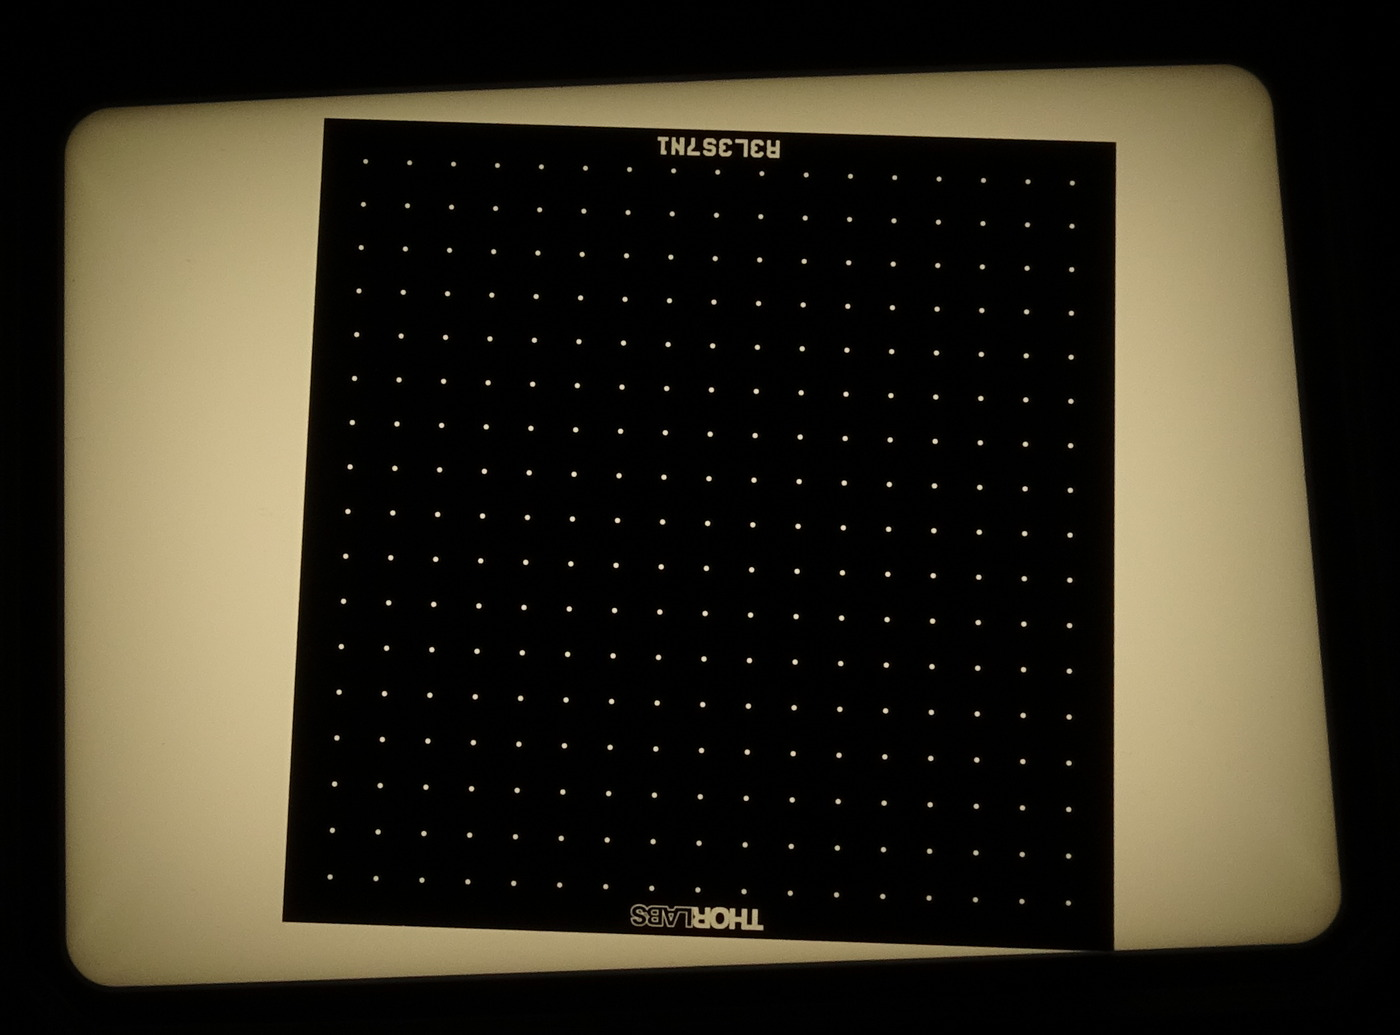
\includegraphics[width=\linewidth]{fig/thorlabs-target.jpg}
  \caption{The Thorlabs R3L3S7N1 target on its LED backlight, from our capture.}
  \label{fig:supp-thorlabs-target}
\end{figure}
\begin{table}[t]
  \centering
  \small
  \begin{tabular}{@{}ll@{}}
    \toprule
    grid & $17\times17$ dots, $80\times80\,\mathrm{mm}$ \\
    dot spacing & $5.000\,\mathrm{mm}$ \\
    dot diameter & $0.500\,\mathrm{mm}$ \\
    tolerance$^{*}$ & $\pm5\,\mathrm{\mu m}$ \\
    substrate & soda-lime glass, $90\times90\,\mathrm{mm}$ \\
    coating & OD\,3 chrome, $0.12\,\mathrm{\mu m}$ \\
    polarity & clear dots, opaque field \\
    \bottomrule
  \end{tabular}
  \caption{Specifications of the Thorlabs R3L3S7N1 target (manufacturer's drawing, 15 Nov 2024). $^{*}$Of the dot diameter, the dot spacing and the corner-to-corner distance.}
  \label{tab:supp-thorlabs-target}
\end{table}

\subsection{Evaluation Protocol}
\label{sec:supp-thorlabs-protocol}
\paragraph{Capture.}
The target is backlit by an LED panel in a dark room, so the dots are the only light in the image. The target is kept fixed, and the camera, mounted on a ball head on a pivot arm, is rotated between the images so that the dots cover the whole image, the rim included. The distance to the target is in the same range as for the Siemens-star and AprilGrid captures of the same lens, and the aperture is the same ($f/22$; $f/32$ for the fisheye at $30\,\mathrm{cm}$), so the defocus is comparable.

\paragraph{Detection.}
We detect the dots with a Förstner blob detector on the full-resolution green image, in which each red and blue photosite is interpolated bilinearly from its green neighbours (the image every geometric detector of our pipeline uses, the Siemens-star front end included), \cite{forstner1987fast} and take the blob centroid as the image of the dot centre. The imaged dots cover a median of 12 to 34\,px$^2$ per set (diameters of 4 to 7\,px, full-resolution pixels) across the image set, so we assume that identifying the blob centroid with the dot centre introduces negligible bias. The imaged dots cover a median of 12 to 34\,px$^2$ per set (diameters of 4 to 7\,px), so identifying the blob centroid with the dot centre introduces negligible bias.

\paragraph{Correspondences.}
In each image, the detected dot centres are assigned to the $17\times17$ grid nodes once, before any model is evaluated: a RANSAC pose of the target with a one-to-one (Hungarian) assignment, in which a detection farther than half the grid spacing ($2.5\,\mathrm{mm}$ on the target) from every node stays unassigned.
These correspondences are the same for every model, and no model rejects dots afterwards.

\paragraph{Motion.}
The camera model under test is held fixed. Since the camera rotates about one unknown pivot, a target point $\vbX$ is in view $k$ at $\vbR_k(\vbX-\vbc)+\vbd$, with a rotation $\vbR_k$ per view and the centre $\vbc$ and the offset $\vbd$ shared by all views ($3N+6$ parameters for $N$ views, instead of $6N$ for free poses). They are fitted by minimizing the robust reprojection error. Constraining the motion in this way keeps the unknown poses from absorbing reprojection error at test time.

\paragraph{Train and test split.}
The grid nodes $(i,j)$ are split by the parity of $i+j$ into two interleaved halves, like the colours of a checkerboard. The motion is fitted on one half and the reprojection error is measured on the other; the halves are then swapped and the errors of both are pooled. Every reported residual is therefore of a dot that did not enter the fit, and both halves cover the whole image, the rim included.

\paragraph{Statistics.}
We report the median, mean, $95$th percentile and RMS of the reprojection error in pixels. A model is evaluated on a dot only if it back-projects the dot and projects its fitted target point; the models of a set are compared on the dots that every one of them evaluates, so all rows of a set rest on the same dots.
A model that is not defined over the whole image, \eg a calibration restricted to the area its detections covered or a parametric distortion that does not reach the rim, leaves out the dots it cannot evaluate, which lie at the image border and are the hardest ones; the common dots then favour such a model. We therefore also computed each model's coverage, the share of the registered dots it evaluates, and its error on all of them. Every model of \cref{tab:refinement-chrome} evaluates at least 99.4\,\% of the registered dots, except the spline start on the fisheye's AprilGrid set (95.0\,\%), whose refinement, estimated over the whole lens coverage, evaluates 99.4\,\%. The median error of a model on all of its dots differs from that on the common dots by at most 0.002\,px, and by at most 6\,\% on the fisheye's AprilGrid set, where the common dots leave out the border.

\paragraph{Confidence intervals.}
We compare two models of a set, \eg a camera after the radiometric refinement and its geometric start, by the difference of a statistic of the reprojection error (median, mean, $95$th percentile or RMS), each computed over the dots that every model of the set evaluates, pooled over all images. The interval of this difference is a paired, nonparametric bootstrap over images. The dots of one image are correlated through its pose, so the image is the resampling unit and not the dot. In each of $10{,}000$ draws, as many images as the set contains are drawn with replacement; the statistic of both models is recomputed on the dots of the drawn images, an image drawn several times counting as often, and their difference is taken. Both models are thus always evaluated on the same images and dots, which removes the variation between images from the comparison. From the $10{,}000$ differences we take the $95\,\%$ bias-corrected and accelerated (BCa) interval \cite{efron1987better}, whose bias correction is the share of draws below the observed difference and whose acceleration is estimated by a jackknife that leaves out one image at a time. The four statistics share the same draws, and the random seed is fixed, so the intervals are reproducible. A difference whose interval excludes zero is significant at the $5\,\%$ level. The intervals are computed over the whole image and, separately, over its centre and its edge (radii below $0.4$ and above $0.6$ of the largest radius).


\paragraph{Results.}
\Cref{tab:supp-refinement-a,tab:supp-refinement-b} give the four statistics of \cref{tab:refinement-chrome} for every camera model, lens and calibration target, with the difference between the radiometric refinement and its geometric start and the 95\,\% interval of this difference.

% The runtime as its own section: its table carries the number A6 although it comes before Tabs. A4 and A5 in the source,
% so that the numbers of Secs. A.1 to A.13 and Tabs. A1 to A5 do not change. The table counter is set back after it.
\section{Runtime}
\label{sec:supp-runtime}
The radiometric refinement of the Sigma 14\,mm Siemens-star set (\timingPhotographs{} photographs of \timingWidth{}\,$\times$\,\timingHeight{}\,px, \timingSamples{} samples each, \timingObservations{} observations per iteration; \timingIterations{} LM iterations over \timingParametersTotal{} free parameters: \timingParametersCamera{} of the camera, \timingParametersPoses{} of the poses, \timingParametersTarget{} of the target and \timingParametersLighting{} of the lighting) takes \timingMeanS{}\,$\pm$\,\timingStdS{}\,s (mean $\pm$ std over \timingRuns{} runs, \timingPerIterationS{}\,s per iteration, writing the calibrated camera included) on one NVIDIA \timingGpu{} with \timingThreads{} CPU threads, from its loaded start; the decoding and the geometric start are excluded. \Cref{tab:supp-runtime} lists the size of the problem.
\begin{table}[h!]
	\centering
	\renewcommand{\thetable}{A6}\renewcommand{\theHtable}{A6}%
	% the generated table is 13 pt wider than a column: set 7 % wider and scaled to the column
	\resizebox{\linewidth}{!}{\begin{minipage}{1.07\linewidth}\footnotesize
\setlength{\tabcolsep}{1.5pt}
\begin{tabular*}{\linewidth}{@{\extracolsep{\fill}}lr@{}}
\toprule
\multicolumn{2}{@{}l}{\underline{\textit{Sigma 14\,mm, Siemens stars, central spline}}} \\
Photographs & 132 at $4256\times2848$\,px \\
Samples per photograph & 16,384 \\
Observations per iteration & 2,162,688 \\
Free parameters (camera / poses / target / lighting) & 1,443 / 792 / 29 / 9 \\
LM iterations & 25 \\
Time per iteration [s] & 26.1 \\
Refinement time [s] (mean $\pm$ std, min--max) & 703.5 $\pm$ 3.7 (700.3--710.5) \\
Runs & 8 \\
GPU, CPU threads & NVIDIA B200, 8 \\
\bottomrule
\end{tabular*}
\end{minipage}}
	\caption{Runtime of one radiometric calibration: the refinement of the central spline of the Sigma 14\,mm lens on the Siemens-star set, from its loaded geometric start to the written calibrated camera, over \timingRuns{} runs, each on its own GPU after an untimed warm-up run. The decoding of the photographs and the geometric start are not included.}
	\label{tab:supp-runtime}
\end{table}
\addtocounter{table}{-1}

\begin{table*}[t]
  \centering
  \scriptsize
\setlength{\tabcolsep}{3pt}
\begin{tabular*}{\linewidth}{@{\extracolsep{\fill}}lrrlrrl@{}}
\toprule
 & \multicolumn{3}{c}{\textbf{Median [px]}} & \multicolumn{3}{c}{\textbf{95th percentile [px]}} \\
\cmidrule(lr){2-4}\cmidrule(lr){5-7}
\textbf{Model} & Geom. & Radiom. & $\Delta$ [95\,\% interval] & Geom. & Radiom. & $\Delta$ [95\,\% interval] \\
\midrule
\multicolumn{7}{@{}l}{\underline{\textit{Tamron 20\,mm, AprilGrid}} (142 test images, 40,999 dots)} \\
Brown--Conrady & 0.119 & \textbf{0.067} & $-0.052$ [$-0.062$, $-0.043$] & 0.356 & \textbf{0.173} & $-0.183$ [$-0.208$, $-0.161$] \\
OpenCV-14 & 0.107 & \textbf{0.060} & $-0.048$ [$-0.059$, $-0.037$] & 0.373 & \textbf{0.155} & $-0.217$ [$-0.270$, $-0.180$] \\
Kannala--Brandt & 0.117 & \textbf{0.106} & $-0.011$ [$-0.020$, $-0.001$] & 0.446 & \textbf{0.285} & $-0.162$ [$-0.220$, $-0.102$] \\
Double Sphere & 0.261 & \textit{0.286} & $+0.025$ [$+0.000$, $+0.046$] & 1.70 & \textbf{1.16} & $-0.545$ [$-0.773$, $-0.294$] \\
Central spline & 0.040 & \textit{0.048} & $+0.008$ [$+0.006$, $+0.010$] & 0.131 & \textbf{0.119} & $-0.012$ [$-0.027$, $-0.002$] \\
\midrule
\multicolumn{7}{@{}l}{\underline{\textit{Tamron 20\,mm, Siemens stars}} (112 test images, 32,170 dots)} \\
Brown--Conrady & 0.288 & \textbf{0.135} & $-0.154$ [$-0.179$, $-0.132$] & 0.855 & \textbf{0.321} & $-0.534$ [$-0.589$, $-0.480$] \\
OpenCV-14 & 0.308 & \textbf{0.131} & $-0.177$ [$-0.203$, $-0.154$] & 0.969 & \textbf{0.337} & $-0.633$ [$-0.704$, $-0.566$] \\
Kannala--Brandt & 0.183 & 0.176 & $-0.007$ [$-0.022$, $+0.005$] & 0.730 & \textbf{0.515} & $-0.215$ [$-0.264$, $-0.164$] \\
Double Sphere & 0.219 & \textit{0.268} & $+0.049$ [$+0.036$, $+0.062$] & 0.717 & \textbf{0.625} & $-0.092$ [$-0.141$, $-0.040$] \\
Central spline & 0.161 & \textbf{0.136} & $-0.026$ [$-0.034$, $-0.017$] & 0.436 & \textbf{0.331} & $-0.105$ [$-0.128$, $-0.084$] \\
\midrule
\multicolumn{7}{@{}l}{\underline{\textit{Sigma 14\,mm, AprilGrid}} (141 test images, 40,744 dots)} \\
Brown--Conrady & 0.499 & \textbf{0.377} & $-0.122$ [$-0.144$, $-0.099$] & 2.07 & \textbf{1.78} & $-0.289$ [$-0.360$, $-0.211$] \\
OpenCV-14 & 0.476 & \textbf{0.359} & $-0.117$ [$-0.146$, $-0.092$] & 2.16 & \textbf{1.74} & $-0.419$ [$-0.543$, $-0.290$] \\
Kannala--Brandt & 0.456 & \textbf{0.351} & $-0.105$ [$-0.125$, $-0.084$] & 1.99 & \textbf{1.79} & $-0.202$ [$-0.308$, $-0.122$] \\
Double Sphere & 1.42 & 1.34 & $-0.081$ [$-0.170$, $+0.000$] & 5.13 & \textbf{4.42} & $-0.707$ [$-1.171$, $-0.334$] \\
Central spline & 0.479 & \textbf{0.331} & $-0.148$ [$-0.189$, $-0.114$] & 2.45 & \textbf{1.76} & $-0.691$ [$-0.895$, $-0.539$] \\
\midrule
\multicolumn{7}{@{}l}{\underline{\textit{Sigma 14\,mm, Siemens stars}} (141 test images, 40,744 dots)} \\
Brown--Conrady & 0.687 & \textbf{0.359} & $-0.328$ [$-0.375$, $-0.284$] & 2.73 & \textbf{1.72} & $-1.009$ [$-1.253$, $-0.790$] \\
OpenCV-14 & 0.600 & \textbf{0.384} & $-0.217$ [$-0.270$, $-0.170$] & 2.87 & \textbf{1.93} & $-0.942$ [$-1.200$, $-0.703$] \\
Kannala--Brandt & 0.567 & \textbf{0.329} & $-0.238$ [$-0.277$, $-0.199$] & 2.37 & \textbf{1.75} & $-0.620$ [$-0.813$, $-0.392$] \\
Double Sphere & 0.734 & \textbf{0.461} & $-0.273$ [$-0.315$, $-0.232$] & 2.42 & \textbf{1.94} & $-0.484$ [$-0.708$, $-0.323$] \\
Central spline & 0.504 & \textbf{0.366} & $-0.137$ [$-0.174$, $-0.104$] & 2.35 & \textbf{1.97} & $-0.375$ [$-0.560$, $-0.229$] \\
\midrule
\multicolumn{7}{@{}l}{\underline{\textit{Sigma 8\,mm fisheye, AprilGrid}} (153 test images, 40,928 dots)} \\
OpenCV-14 & 1.98 & \textbf{1.70} & $-0.285$ [$-0.406$, $-0.177$] & 9.15 & \textbf{5.68} & $-3.472$ [$-3.825$, $-3.029$] \\
Kannala--Brandt & 2.00 & \textbf{1.52} & $-0.479$ [$-0.560$, $-0.395$] & 6.80 & \textbf{5.43} & $-1.371$ [$-1.564$, $-1.207$] \\
Double Sphere & 2.09 & \textbf{1.49} & $-0.600$ [$-0.671$, $-0.538$] & 7.41 & \textbf{5.45} & $-1.965$ [$-2.126$, $-1.842$] \\
Central spline & 1.99 & \textbf{1.45} & $-0.543$ [$-0.654$, $-0.433$] & 7.58 & \textbf{5.51} & $-2.076$ [$-2.491$, $-1.702$] \\
\midrule
\multicolumn{7}{@{}l}{\underline{\textit{Sigma 8\,mm fisheye, Siemens stars}} (82 test images, 22,973 dots)} \\
OpenCV-14 & 0.123 & \textbf{0.079} & $-0.044$ [$-0.065$, $-0.025$] & 0.818 & \textbf{0.440} & $-0.378$ [$-0.584$, $-0.224$] \\
Kannala--Brandt & 0.113 & \textbf{0.063} & $-0.050$ [$-0.066$, $-0.037$] & 0.590 & \textbf{0.254} & $-0.336$ [$-0.437$, $-0.237$] \\
Double Sphere & 0.109 & \textbf{0.067} & $-0.042$ [$-0.059$, $-0.029$] & 0.591 & \textbf{0.289} & $-0.302$ [$-0.391$, $-0.238$] \\
Central spline & 0.121 & \textbf{0.100} & $-0.020$ [$-0.039$, $-0.002$] & 0.996 & \textbf{0.538} & $-0.458$ [$-0.717$, $-0.309$] \\
\bottomrule
\end{tabular*}

  \caption{Median and $95$th percentile of the reprojection error on the held-out target at the geometric start and after the radiometric refinement, with their difference $\Delta$ and its 95\,\% bootstrap interval. Bold: significantly lower than the start; italic: significantly higher.}
  \label{tab:supp-refinement-a}
\end{table*}
\begin{table*}[t]
  \centering
  \scriptsize
\setlength{\tabcolsep}{3pt}
\begin{tabular*}{\linewidth}{@{\extracolsep{\fill}}lrrlrrl@{}}
\toprule
 & \multicolumn{3}{c}{\textbf{Mean [px]}} & \multicolumn{3}{c}{\textbf{RMS [px]}} \\
\cmidrule(lr){2-4}\cmidrule(lr){5-7}
\textbf{Model} & Geom. & Radiom. & $\Delta$ [95\,\% interval] & Geom. & Radiom. & $\Delta$ [95\,\% interval] \\
\midrule
\multicolumn{7}{@{}l}{\underline{\textit{Tamron 20\,mm, AprilGrid}} (142 test images, 40,999 dots)} \\
Brown--Conrady & 0.147 & \textbf{0.077} & $-0.069$ [$-0.080$, $-0.059$] & 0.185 & \textbf{0.092} & $-0.093$ [$-0.110$, $-0.081$] \\
OpenCV-14 & 0.144 & \textbf{0.070} & $-0.075$ [$-0.090$, $-0.063$] & 0.201 & \textbf{0.083} & $-0.118$ [$-0.145$, $-0.098$] \\
Kannala--Brandt & 0.159 & \textbf{0.124} & $-0.034$ [$-0.052$, $-0.020$] & 0.214 & \textbf{0.149} & $-0.065$ [$-0.092$, $-0.043$] \\
Double Sphere & 0.473 & \textbf{0.429} & $-0.044$ [$-0.085$, $-0.007$] & 0.875 & \textbf{0.696} & $-0.179$ [$-0.228$, $-0.128$] \\
Central spline & 0.051 & \textit{0.055} & $+0.003$ [$+0.001$, $+0.006$] & 0.067 & 0.065 & $-0.002$ [$-0.007$, $+0.001$] \\
\midrule
\multicolumn{7}{@{}l}{\underline{\textit{Tamron 20\,mm, Siemens stars}} (112 test images, 32,170 dots)} \\
Brown--Conrady & 0.350 & \textbf{0.151} & $-0.199$ [$-0.225$, $-0.177$] & 0.430 & \textbf{0.176} & $-0.253$ [$-0.282$, $-0.228$] \\
OpenCV-14 & 0.386 & \textbf{0.152} & $-0.234$ [$-0.261$, $-0.209$] & 0.483 & \textbf{0.181} & $-0.302$ [$-0.333$, $-0.273$] \\
Kannala--Brandt & 0.257 & \textbf{0.213} & $-0.044$ [$-0.061$, $-0.028$] & 0.342 & \textbf{0.261} & $-0.081$ [$-0.103$, $-0.060$] \\
Double Sphere & 0.279 & 0.296 & $+0.017$ [$-0.001$, $+0.033$] & 0.358 & 0.344 & $-0.013$ [$-0.036$, $+0.008$] \\
Central spline & 0.190 & \textbf{0.153} & $-0.037$ [$-0.045$, $-0.029$] & 0.230 & \textbf{0.180} & $-0.050$ [$-0.060$, $-0.041$] \\
\midrule
\multicolumn{7}{@{}l}{\underline{\textit{Sigma 14\,mm, AprilGrid}} (141 test images, 40,744 dots)} \\
Brown--Conrady & 0.716 & \textbf{0.568} & $-0.148$ [$-0.168$, $-0.128$] & 0.997 & \textbf{0.825} & $-0.172$ [$-0.201$, $-0.146$] \\
OpenCV-14 & 0.712 & \textbf{0.544} & $-0.168$ [$-0.198$, $-0.142$] & 1.02 & \textbf{0.791} & $-0.233$ [$-0.284$, $-0.191$] \\
Kannala--Brandt & 0.671 & \textbf{0.542} & $-0.128$ [$-0.147$, $-0.110$] & 0.956 & \textbf{0.802} & $-0.154$ [$-0.185$, $-0.126$] \\
Double Sphere & 1.95 & \textbf{1.80} & $-0.145$ [$-0.237$, $-0.061$] & 2.88 & \textbf{2.59} & $-0.298$ [$-0.387$, $-0.210$] \\
Central spline & 0.770 & \textbf{0.530} & $-0.240$ [$-0.288$, $-0.199$] & 1.22 & \textbf{0.797} & $-0.428$ [$-0.525$, $-0.343$] \\
\midrule
\multicolumn{7}{@{}l}{\underline{\textit{Sigma 14\,mm, Siemens stars}} (141 test images, 40,744 dots)} \\
Brown--Conrady & 0.968 & \textbf{0.546} & $-0.422$ [$-0.485$, $-0.367$] & 1.42 & \textbf{0.796} & $-0.625$ [$-0.761$, $-0.512$] \\
OpenCV-14 & 0.942 & \textbf{0.598} & $-0.344$ [$-0.405$, $-0.288$] & 1.50 & \textbf{0.884} & $-0.611$ [$-0.736$, $-0.503$] \\
Kannala--Brandt & 0.825 & \textbf{0.515} & $-0.310$ [$-0.360$, $-0.263$] & 1.23 & \textbf{0.767} & $-0.459$ [$-0.570$, $-0.361$] \\
Double Sphere & 0.926 & \textbf{0.650} & $-0.276$ [$-0.324$, $-0.235$] & 1.17 & \textbf{0.905} & $-0.262$ [$-0.333$, $-0.206$] \\
Central spline & 0.780 & \textbf{0.594} & $-0.186$ [$-0.235$, $-0.148$] & 1.20 & \textbf{0.901} & $-0.301$ [$-0.403$, $-0.226$] \\
\midrule
\multicolumn{7}{@{}l}{\underline{\textit{Sigma 8\,mm fisheye, AprilGrid}} (153 test images, 40,928 dots)} \\
OpenCV-14 & 2.98 & \textbf{2.18} & $-0.801$ [$-0.963$, $-0.651$] & 4.14 & \textbf{2.80} & $-1.336$ [$-1.536$, $-1.144$] \\
Kannala--Brandt & 2.59 & \textbf{2.01} & $-0.578$ [$-0.649$, $-0.506$] & 3.33 & \textbf{2.65} & $-0.682$ [$-0.750$, $-0.614$] \\
Double Sphere & 2.75 & \textbf{1.99} & $-0.763$ [$-0.830$, $-0.698$] & 3.59 & \textbf{2.64} & $-0.949$ [$-1.023$, $-0.878$] \\
Central spline & 2.70 & \textbf{1.96} & $-0.746$ [$-0.868$, $-0.638$] & 3.69 & \textbf{2.63} & $-1.059$ [$-1.306$, $-0.897$] \\
\midrule
\multicolumn{7}{@{}l}{\underline{\textit{Sigma 8\,mm fisheye, Siemens stars}} (82 test images, 22,973 dots)} \\
OpenCV-14 & 0.280 & \textbf{0.164} & $-0.115$ [$-0.188$, $-0.077$] & 2.62 & \textbf{1.09} & $-1.533$ [$-2.953$, $-0.132$] \\
Kannala--Brandt & 0.182 & \textbf{0.089} & $-0.093$ [$-0.122$, $-0.070$] & 0.265 & \textbf{0.123} & $-0.141$ [$-0.181$, $-0.107$] \\
Double Sphere & 0.181 & \textbf{0.098} & $-0.083$ [$-0.109$, $-0.064$] & 0.265 & \textbf{0.151} & $-0.114$ [$-0.148$, $-0.086$] \\
Central spline & 0.256 & \textbf{0.182} & $-0.074$ [$-0.113$, $-0.042$] & 0.472 & 0.502 & $+0.029$ [$-0.153$, $+0.342$] \\
\bottomrule
\end{tabular*}

  \caption{Mean and RMS of the reprojection error, as \cref{tab:supp-refinement-a}.}
  \label{tab:supp-refinement-b}
\end{table*}
